\documentclass[11pt]{article}
\usepackage[scaled=0.92]{helvet}
\usepackage{geometry}
\geometry{letterpaper,tmargin=1in,bmargin=1in,lmargin=1in,rmargin=1in}
\usepackage[parfill]{parskip} % Activate to begin paragraphs with an empty line rather than an indent %\usepackage{graphicx}
\usepackage{amsmath,amssymb, mathrsfs,  mathtools, dsfont}
\usepackage{tabularx}
\usepackage{tikz-cd}
\usepackage[font=footnotesize,labelfont=bf]{caption}
\usepackage{graphicx}
\usepackage{xcolor}
%\usepackage[linkbordercolor ={1 1 1} ]{hyperref}
%\usepackage[sf]{titlesec}
\usepackage{natbib}
\usepackage{../../Tianpei_Report}

%\usepackage{appendix}
%\usepackage{algorithm}
%\usepackage{algorithmic}

%\renewcommand{\algorithmicrequire}{\textbf{Input:}}
%\renewcommand{\algorithmicensure}{\textbf{Output:}}



\begin{document}
\title{Lecture 5: Submanifolds}
\author{ Tianpei Xie}
\date{Oct. 17th., 2022}
\maketitle
\tableofcontents
\newpage
\section{Embedded Submanifolds}
\subsection{Defintions and Examples}
\begin{itemize}
\item \begin{definition}
Suppose $M$ is a smooth manifold with or without boundary. \emph{\textbf{An \underline{embedded} \underline{submanifold}}} of $M$ is a subset $S \subseteq M$ that is a \emph{manifold} (without boundary) in the \emph{\textbf{subspace topology}}, endowed with a \emph{\textbf{smooth structure}} with respect to which the \emph{\textbf{inclusion map}} $S \xhookrightarrow{} M$ is a \underline{\emph{\textbf{smooth embedding}}}. Embedded submanifolds are also called \emph{\textbf{regular submanifolds}}.
\end{definition}

\item \begin{definition}
If $S$ is an \emph{embedded submanifold} of $M$, the \emph{\textbf{difference}} $\text{dim }M - \text{dim }S$ is called
\underline{\emph{\textbf{the codimension}}} of $S$ in $M$, and the \emph{\textbf{containing manifold}} $M$ is called \emph{\textbf{the \underline{ambient} manifold}} for $S$. 

An embedded \emph{\textbf{hypersurface}} is an embedded submanifold of codimension $1$. The \emph{empty set} is an embedded submanifold of \emph{any dimension}.
\end{definition}

\item \begin{proposition}(\textbf{Open Submanifolds}). \citep{lee2003introduction}\\
Suppose $M$ is a smooth manifold. The embedded submanifolds of \textbf{codimension 0} in $M$ are exactly the \textbf{open submanifolds}.
\end{proposition}

\item There are several other ways to create submanifolds:
\begin{proposition} (\textbf{Images of Embeddings as Submanifolds}). \citep{lee2003introduction} \\
Suppose $M$ is a smooth manifold with or without boundary, $N$ is a smooth manifold, and $F: N \rightarrow M$ is a \textbf{smooth embedding}. Let $S = F(N)$. With the subspace topology, $S$ is a topological manifold, and it has a \textbf{unique smooth structure} making it into an \textbf{embedded submanifold} of $M$ with the property that $F$ is a \textbf{diffeomorphism} onto its image.
\end{proposition}

\item \begin{proposition} (\textbf{Slices of Product Manifolds}). \citep{lee2003introduction}\\
Suppose $M$ and $N$ are smooth manifolds. For each $p \in N$, the subset $M \times \set{p}$ (called \textbf{a slice of the product manifold}) is an \textbf{embedded submanifold} of $M \times N$ diffeomorphic to $M$.
\end{proposition}

\item \begin{proposition} (\textbf{Graphs as Submanifolds}). \citep{lee2003introduction}\\
Suppose $M$ is a smooth $m$-manifold (without boundary), $N$ is a smooth $n$-manifold with or without boundary, $U \subseteq M$ is open, and $f: U \rightarrow N$ is a smooth map. Let $\Gamma(f) \subseteq M \times N$ denote \textbf{the graph of $f$}:
\begin{align*}
\Gamma(f) &= \set{ (x,y) \in M \times N: x \in U, y = f(x)}.
\end{align*} Then $\Gamma(f)$ is an \textbf{embedded $m$-dimensional} submanifold of $M \times N$
\end{proposition}

\item \begin{definition}
An embedded submanifold $S \subseteq M$ is said to be \underline{\emph{\textbf{properly embedded}}} if the inclusion $S \xhookrightarrow{} M$ is a \emph{\textbf{proper map}}.
\end{definition}

\item \begin{proposition}
Suppose $M$ is a smooth manifold with or without boundary and $S \subseteq M$ is an embedded submanifold. Then $S$ is \textbf{properly} embedded if and only if it
is a \textbf{closed} subset of $M$.
\end{proposition}

\item \begin{corollary}
Every \textbf{compact} embedded submanifold is \textbf{properly} embedded.
\end{corollary}

\item \begin{proposition} (\textbf{Global Graphs Are Properly Embedded}). \citep{lee2003introduction}\\
Suppose $M$ is a smooth manifold, $N$ is a smooth manifold with or without boundary, and $f: M \rightarrow N$ is a \textbf{smooth} map. With the smooth manifold structure as above, the graph of $f$ $\Gamma(f)$ is properly embedded in $M \times N$.
\end{proposition}
\end{itemize}
\subsection{Slice Charts for Embedded Submanifolds}
\begin{itemize}
\item \begin{definition}
if $U$ is an open subset of $\bR^n$ and $k\in \set{0,\ldots,n}$, a \underline{\emph{\textbf{$k$-dimensional slice}}} of $U$ (or simply a $k$-slice) is any subset of the form 
\begin{align*}
S = \set{(x^1,\ldots,x^k, x^{k+1},\ldots, x^n) \in U: x^{k+1} = c^{k+1},\ldots, x^n = c^n}
\end{align*} for some constants $c^{k+1},\ldots,c^n$. (When $k = n$, this just means $S = U$.)  Clearly, \emph{\textbf{every $k$-slice is \underline{homeomorphic to an open subset of $\bR^k$}}}. 
\end{definition}

\item \begin{remark}
Sometimes it is convenient to consider slices defined by setting some subset of the coordinates other than the last ones equal to constants.
\end{remark}

\item \begin{remark}
Although in general we allow our slices to be defined by arbitrary constants $c^{k+1},\ldots,c^n$, it is sometimes useful to have slice coordinates for which the constants are \emph{\textbf{all zero}}, which can easily be achieved by subtracting a constant from each coordinate function.
\end{remark}

\item \begin{definition}
Let $M$ be a smooth $n$-manifold, and let $(U, \varphi)$ be \underline{a smooth chart \textbf{on $M$}}. If $S$ is a subset of $U$ such that $\varphi(S)$ is a $k$-slice of $\varphi(U)$, then we say that \underline{\emph{\textbf{$S$ is a $k$-slice of $U$}}}. 
\end{definition}

\item \begin{definition}
Given a subset $S \subseteq M$ and a nonnegative integer $k$, we say that \emph{\textbf{$S$ satisfies the local $k$-slice condition}} if \emph{each point} of $S$ is contained
in the domain of a smooth chart  $(U, \varphi)$ for $M$ such that \emph{\underline{$S \cap U$} is a \textbf{single $k$-slice} in $U$}. Any such chart is called \emph{\textbf{a slice chart for $S$ in $M$}} , and the corresponding coordinates $(x^1,\ldots,x^n)$ are called \emph{\textbf{slice coordinates}}.
\end{definition}

\begin{figure}
\begin{minipage}[htb]{1\linewidth}
  \centering
  \centerline{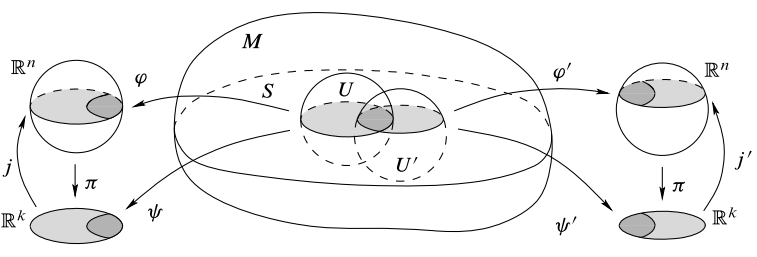
\includegraphics[scale = 0.45]{smooth_compatiability_slice_chart.png}}
\end{minipage}
\caption{\footnotesize{\textbf{Smooth compatibility of slice charts  \citep{lee2003introduction}}}}
\label{fig: smooth_compatiability_slice_chart}
\end{figure}


\item \begin{remark}
The key to understand the \underline{\emph{\textbf{the local $k$-slice condition}}} for $S \subseteq M$:
\begin{enumerate}
\item It is a condition on the \emph{\textbf{subset}} $S$ only; it does \emph{\textbf{not presuppose}} any particular \emph{\textbf{topology}} or \emph{\textbf{smooth structure}} on $S$. All it needs is the topology and smooth structure from the ambient manifold $M$.
\item The \emph{local neighborhood} $U \subseteq M$ is a \underline{\emph{\textbf{neighborhood} of $p$ in the \textbf{ambient manifold $M$}}} not a neigborhood in $S$ (since we do not define such topology);
\item The $k$-slice representation is for the \emph{\textbf{intersection}} \underline{$S\cap U$} under \emph{\textbf{the smooth chart}} $(U, \varphi)$ of \emph{\textbf{the ambient manifold $M$.}}
\end{enumerate}
\end{remark}

\item \begin{theorem}\label{thm: local_slice_emb_subman} (\textbf{Local Slice Criterion for Embedded Submanifolds})  \citep{lee2003introduction}.\\
Let $M$ be a smooth $n$-manifold. If $S \subseteq M$ is an embedded $k$-dimensional submanifold, then $S$ satisfies the local $k$-slice condition. \textbf{Conversely}, if $S \subseteq M$ is a subset that \textbf{satisfies the local $k$-slice condition}, then with the \textbf{subspace topology}, $S$ is a topological manifold of dimension $k$, and it \textbf{has a smooth structure} making it into a $k$-dimensional embedded submanifold of $M$ .
\end{theorem}

\item \begin{theorem}
If $M$ is a smooth $n$-manifold with boundary, then with the subspace topology, $\partial M$ is a topological $(n-1)$-dimensional manifold (without boundary), and has a smooth structure such that it is a properly \textbf{embedded submanifold} of $M$.
\end{theorem}

\item \begin{example} (\emph{\textbf{Spheres as Submanifolds}}).\\
For any $n \ge 0$, \emph{\textbf{$\bS^n$ is an embedded submanifold of $\bR^{n+1}$}}, because it is \emph{locally} the \emph{graph} of \emph{a smooth function}:  the intersection of $\bS^n$ with the open subset $\set{x: x^i > 0}$ is the graph of the smooth function
\begin{align*}
x^i &= f(x^1,\ldots,x^{i-1}, x^{i+1},\ldots,x^{n+1}),
\end{align*} where $f: \bB^n \rightarrow \bR$ is given by $f(u) = \sqrt{1 - \abs{u}^2}$. Similarly, the intersection of $\bS^n$ with $\set{x: x^i < 0}$ is the graph of $-f$. Since every point in $\bS^n$ is in one of these sets, $\bS^n$ satisfies the local $n$-slice condition and is thus an embedded submanifold of $\bR^{n+1}$. 
\end{example}
\end{itemize}

\subsection{Level Sets}
\begin{itemize}
\item \begin{remark}
In practice, embedded submanifolds are most often presented as \emph{\textbf{solution sets}} of \emph{equations or systems of equations}.
\end{remark}

\begin{figure}
\begin{minipage}[htb]{1\linewidth}
  \centering
  \centerline{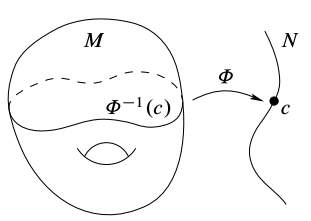
\includegraphics[scale = 0.45]{level_sets.png}}
\end{minipage}
\caption{\footnotesize{\textbf{A level set  \citep{lee2003introduction}}}}
\label{fig: level_sets}
\end{figure}

\item \begin{definition}
If $\Phi: M \rightarrow N$ is any map and $c$ is any point of N, we call the set \emph{\textbf{$\Phi^{-1}(c)$ a level set of $\Phi$}} (Fig. \ref{fig: level_sets}). (In the special case $N = \bR^k$ and $c = 0$, the level set $\Phi^{-1}(0)$ is usually called \emph{\textbf{the zero set of $\Phi$}}.)
\end{definition}

\item \begin{remark}
It is easy to find \emph{level sets of smooth functions} that are \emph{not smooth submanifolds}. 
\begin{align*}
\Theta(x,y)  = x^2 - y, \quad \Phi(x,y) = x^2 - y^2, \quad  \Psi(x, y) = x^2 -y^3.
\end{align*} (Note that the zero set $\Theta^{-1}(0)$ is an embedded submanifolds in $\bR^{2}$ but not for others.) In fact, \emph{\textbf{every closed subset of $M$}} can be expressed as \emph{\textbf{the zero set}} of some smooth real-valued function.
\end{remark}

\item \begin{theorem} (\textbf{Constant-Rank Level Set Theorem}). \citep{lee2003introduction} \\
Let $M$ and $N$ be smooth manifolds, and let $\Phi: M \rightarrow N$ be a smooth map \textbf{with constant rank $r$}. \textbf{Each level set} of $\Phi$ is a properly embedded submanifold of \textbf{codimension $r$} in $M$.
\end{theorem}
\begin{proof}
Write $m = \text{dim }M$, $n = \text{dim }N$, and $k = m - r$. Let $c \in \bN$ be arbitrary, and let $S$ denote the level set $\Phi^{-1}(c) \subseteq M$. From the rank theorem, for each $p \in S$ there are smooth charts $(U, \varphi)$ centered at $p$ and $(V, \psi)$ centered at $c = \Phi(p)$ in which $\Phi$ has a coordinate representation of the form (4.1), and therefore $S \cap U$ is the slice
\begin{align*}
\set{(x^1,\ldots,x^r, x^{r+1},\ldots,x^m) \in U:  x^1 = \ldots = x^r = 0}
\end{align*}
Thus $S$ satisfies the local $k$-slice condition, so it is an embedded submanifold of dimension $k$. It is closed in $M$ by continuity, so it is properly embedded by Proposition \ref{thm: local_slice_emb_subman}. \qed 
\end{proof}

\item \begin{corollary} (\textbf{Submersion Level Set Theorem}). \citep{lee2003introduction} \\
 If $M$ and $N$ are smooth manifolds and $\Phi: M \rightarrow N$ is a \textbf{smooth submersion}, then each level set of $\Phi$ is a \textbf{properly embedded} submanifold whose \textbf{codimension} is equal to the \textbf{dimension of $N$}.
\end{corollary}

\item \begin{remark}
This result should be compared to the corresponding result in linear algebra: if $L: \bR^m \rightarrow \bR^r$ is a surjective linear map, then the kernel of $L$ is a linear subspace of codimension $r$ by \emph{\textbf{the rank-nullity law}}.  The vector equation $Lx = 0$ is equivalent to $r$ linearly independent scalar equations, each of which can be thought of as cutting down one of the degrees of freedom in $\bR^m$, leaving a subspace of codimension $r$. 

In the context of smooth manifolds, the analogue of \emph{a surjective linear map} is \emph{\textbf{a smooth submersion}}, \emph{\textbf{each}} of whose \emph{\textbf{(local) component functions cuts down the dimension by one}}.
\end{remark}


\item \begin{definition}
If $\Phi: M \rightarrow N$ is a smooth map, a point $p \in M$ is said to be \underline{\emph{\textbf{a regular point}}} of $\Phi$ if $d\Phi_{p}: T_{p}M \rightarrow
T_{\Phi(p)}N$ is \emph{\textbf{surjective}}; it is \underline{\emph{\textbf{a critical point}}} of $\Phi$ otherwise. 

This means, in particular, that \emph{\textbf{every point}} of $M$ is \emph{\textbf{critical}} if \underline{$\text{dim }M < \text{dim }N$}, and every point is \emph{\textbf{regular}} if and only if $\Phi$ is a \emph{\textbf{submersion}}. 
\end{definition}


\begin{figure}
\begin{minipage}[htb]{1\linewidth}
  \centering
  \centerline{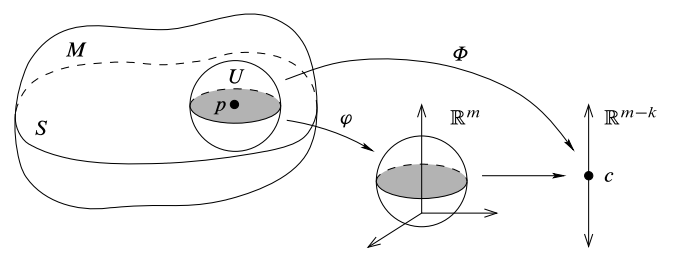
\includegraphics[scale = 0.45]{embedded_subman_local_level_set.png}}
\end{minipage}
\caption{\footnotesize{\textbf{An embedded submanifold is locally a level set \citep{lee2003introduction}}}}
\label{fig: embedded_subman_local_level_set}
\end{figure}

\item \begin{definition}
A point $c \in N$ is said to be \emph{\textbf{a regular value}} of  $\Phi$ if \emph{\textbf{every point} of the level set $\Phi^{-1}(c)$  is a regular point}, and \emph{\textbf{a critical value}} otherwise. In particular, if $\Phi^{-1}(c) = \emptyset$, then $c$ is \emph{a regular value}. Finally, a level set $\Phi^{-1}(c)$  is called \emph{\textbf{a regular level set}} if $c$ is a regular value of $\Phi$; in other words, a regular level set is a level set consisting \emph{\textbf{entirely} of regular points} of $\Phi$ (points $p$ such that $d\Phi_{p}$ is surjective).
\end{definition}

\item \begin{remark}
If $\Phi$ is a \emph{\textbf{smooth immersion}}, \emph{every point is a critical point of $\Phi$}. A level set from a smooth immersion is a critical level set. 
\end{remark}

\item \begin{remark}
\emph{Every properly embedded submanifold $M = \Phi^{-1}(c)$ is a regular level set}. The following theorem shows that the converse is true as well. 
\end{remark}

\item \begin{theorem} (\textbf{Regular Level Set Theorem}).  \citep{lee2003introduction}\\
\textbf{Every regular level set} of a smooth map between smooth manifolds is a \textbf{properly embedded} submanifold whose codimension is equal to the dimension of the codomain.
\end{theorem}

\item \begin{example} (\emph{\textbf{Spheres}}). Now we can give a much easier proof that $\bS^n$ is an embedded submanifold of $\bR^{n+1}$. The sphere is a regular level set of the smooth function $f: \bR^{n+1} \rightarrow \bR$ given by $f(x) = \abs{x}^2$, since $df_x(v) = 2\sum_i x^i v^i$, which is
surjective except at the origin.
\end{example}



\item \begin{proposition} (\textbf{Local Level Set Criterion for Smooth Embedded Submanifolds})\\
Let $S$ be a subset of a smooth $m$-manifold $M$. Then $S$ is an \textbf{embedded $k$-submanifold} of $M$ if and only if every point of $S$ has \textbf{a neighborhood
\underline{$U$ in $M$}} such that \underline{$U \cap S$} is a \textbf{level set} of a \textbf{smooth submersion} $\Phi: U \rightarrow \bR^{m-k}$.
\end{proposition}

\item \begin{definition}
If $S \subseteq M$ is an embedded submanifold, \emph{a smooth map} $\Phi: M \rightarrow N$ such that $S$ is \emph{\textbf{a regular level set of $\Phi$}} is called \underline{\emph{\textbf{a defining map for S}}}. In the special case $N = \bR^{m-k}$ (so that $\Phi$ is a real-valued or vector-valued function), it is usually called \emph{\textbf{a defining function}}. 

More generally, if $U$ is an open subset of $M$ and $\Phi: U \rightarrow N$ is a smooth map such that $S \cap U$ is a regular level set of $\Phi$, then $\Phi$ is called \emph{\textbf{a local defining map (or local defining function) for $S$}}.
\end{definition}

\begin{remark}
The above proposition says \emph{every embedded submanifold admits a local defining function in a neighborhood of each of its points}.
\end{remark}

\begin{figure}
\begin{minipage}[htb]{1\linewidth}
  \centering
  \centerline{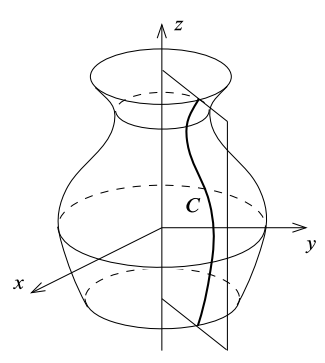
\includegraphics[scale = 0.45]{surface_of_revolution.png}}
\end{minipage}
\caption{\footnotesize{\textbf{A surface of revolution \citep{lee2003introduction}}}}
\label{fig: surface_of_revolution}
\end{figure}


\item \begin{example} (\emph{\textbf{Surfaces of Revolution}}).\\
Let $\bH$ be the half-plane $\set{(r,z): r > 0}$, and suppose $C \subseteq \bH$ is an \emph{\textbf{embedded $1$-dimensional submanifold}}. The \underline{\emph{\textbf{surface of revolution determined by $C$}}} is the subset $S_{C}\subseteq \bR^3$ given by
\begin{align*}
S_{C} &= \set{(x, y, z): \paren{\sqrt{x^2 + y^2}, z} \in C}.
\end{align*} The set $C$ is called its \underline{\emph{\textbf{generating curve}}} (see Fig. \ref{fig: surface_of_revolution}). If $\varphi: U \rightarrow \bR$ is any \emph{\textbf{local defining function}} for $C$ in $\bH$, we get a \emph{\textbf{local defining function}} $\Phi$ for $S_C$ by
\begin{align*}
\Phi(x, y, z) &= \varphi\paren{\sqrt{x^2 + y^2}, z},
\end{align*} defined on the open subset 
\begin{align*}
\widetilde{U} &= \set{(x, y, z): \paren{\sqrt{x^2 + y^2}, z} \in U} \subseteq \bR^{3}
\end{align*}

A computation shows that the Jacobian matrix of $\Phi$ is
\begin{align*}
D\Phi(x, y, z) &= \paren{\frac{x}{r}\partdiff{\varphi}{r}(r, z), \frac{y}{r}\partdiff{\varphi}{r}(r, z), \partdiff{\varphi}{z}(r, z)}
\end{align*} where we have written $r = \sqrt{x^2 + y^2}$.  At any point $(x, y, z) \in S_C$, at least one of the components of $D\Phi(x, y, z)$ is \emph{nonzero}, so \emph{\textbf{$S_C$ is a regular level set of $\Phi$}} and is thus \emph{\textbf{an embedded $2$-dimensional submanifold of $\bR^3$}}.

For a specific example, the \emph{doughnut-shaped \textbf{torus}} of revolution $D$ is the \emph{surface of revolution} obtained from the circle $(r-2)^2 +
z^2 = 1$. It is a regular level set of the function $\Phi(x,y,z) = (\sqrt{x^2 + y^2}-2)^2 + z^2$, which is smooth on $\bR^3$ minus the $z$-axis. \qed
\end{example}

\end{itemize}


\section{Immersed Submanifolds}
\subsection{Definitions and Examples}
\begin{itemize}
\item \begin{definition}
Let $M$ be a smooth manifold with or without boundary. \textit{\textbf{An \underline{immersed} submanifold}} of $M$ is a subset $S \subseteq M$ endowed with a \emph{topology} (\emph{\textbf{not necessarily the subspace topology}}) with respect to which it is \emph{\textbf{a topological manifold}} (without boundary), and \emph{a smooth structure} with respect to which \emph{\textbf{the inclusion map}} $S \xhookrightarrow{} M$ is \emph{\textbf{a smooth immersion}}. 

As for embedded submanifolds, we define the \emph{\textbf{codimension}} of $S$ in $M$ to be $\text{dim }M - \text{dim }S$. 
\end{definition}

\begin{remark}
This terms can be generalized to the \emph{\textbf{immersed topological submanifold of $M$}} to be a subset $S \subseteq M$ endowed with a topology such that it is a topological manifold and such that the \emph{inclusion map is a topological immersion}. It is an \emph{\textbf{embedded topological submanifold}} if the inclusion is a \emph{topological embedding}. 
\end{remark}

\item \begin{remark}
\emph{Every embedded submanifold is also an immersed submanifold}. Because immersed submanifolds are the more general of the two types of submanifolds, we adopt the convention that the term \emph{\textbf{smooth submanifold}} without further qualification means an immersed one, which includes an embedded submanifold as a special case. Similarly, the term \emph{\textbf{smooth hypersurface}} without qualification means an immersed submanifold of \emph{\textbf{codimension $1$}}.
\end{remark}

\item The immersed submanifolds arise in natural way:
\begin{proposition} (\textbf{Images of Immersions as Submanifolds}). \citep{lee2003introduction} \\
Suppose $M$ is a smooth manifold with or without boundary, $N$ is a smooth manifold, and $F: N \rightarrow M$ is an \textbf{injective smooth immersion}. Let $S = F(N)$. Then $S$ has a unique topology and smooth structure such that it is a \textbf{smooth submanifold} of $M$ and such that $F: N \rightarrow S$ is a \textbf{diffeomorphism} onto its image.
\end{proposition}

\item \begin{example} (\emph{\textbf{Immersed Submanifold but Not an Embedded Submanifold}})\\
Both examples of \emph{\textbf{The Figure-Eight}} and \emph{\textbf{the Dense Curve on the Torus}} are \emph{images of injective smooth immersions}, they are \emph{\textbf{immersed submanifolds}} when given appropriate topologies and smooth structures. As smooth manifolds, they are \emph{\textbf{diffeomorphic}} to $\bR$. \emph{They are \textbf{not embedded submanifolds}}, because \emph{\textbf{neither}} one has \emph{\textbf{the subspace topology}}. In fact, their image sets cannot be made into embedded submanifolds even if we are allowed to change their topologies and smooth structures. \qed
\end{example}

\item \begin{remark}
Suppose $M$ is a smooth manifold and $S \subseteq M$ is \emph{\textbf{an immersed submanifold}}. It can be shown that every subset of $S$ that is \emph{\textbf{open}} in the \emph{\textbf{subspace topology}} is also \emph{\textbf{open}} in its given \emph{\textbf{submanifold topology}}; and the \textbf{converse} is true if and only if $S$ is \textbf{\emph{embedded}}.
\end{remark}

\item \begin{proposition} (\textbf{Criterion for Immersed Submanifold to be Embedded Submanifold})\\
Suppose $M$ is a smooth manifold with or without boundary, and $S \subseteq M$ is an \textbf{immersed submanifold}. If any of the following holds, then $S$ is \textbf{embedded}.
\begin{enumerate}
\item $S$ has \textbf{codimension} $0$ in $M$.
\item The inclusion map $S \xhookrightarrow{} M$ is \textbf{proper}.
\item  $S$ is \textbf{compact}.
\end{enumerate}
\end{proposition}

\begin{figure}
\begin{minipage}[htb]{1\linewidth}
  \centering
  \centerline{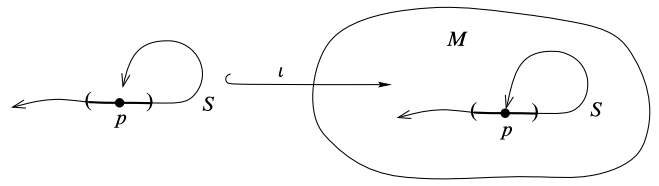
\includegraphics[scale = 0.4]{immersed_subman_locally_embedded.png}}
\end{minipage}
\caption{\footnotesize{\textbf{An immersed submanifold is locally embedded submanifold. \citep{lee2003introduction}}}}
\label{fig: immersed_subman_locally_embedded}
\end{figure}



\item \begin{proposition} (\textbf{Immersed Submanifolds Are Locally Embedded}). \citep{lee2003introduction} \\
If $M$ is a smooth manifold with or without boundary, and $S \subseteq M$ is an \textbf{immersed submanifold}, then for each $p \in S$ there exists a neighborhood $U$ of $p$ \underline{\textbf{in $S$}} that is an \textbf{embedded submanifold} of $M$.
\end{proposition} Note that a smooth immersion is locally a smooth embedding.

\item \begin{remark}
It is important to be clear about what this proposition does and does not say: given an immersed submanifold $S \subseteq M$ and a point $p \in S$,  it is possible to find \emph{a neighborhood $U$ of $p$ \underline{\textbf{in $S$}}} such that \underline{$U$} is \emph{embedded}; but it may not be possible to find \emph{a neighborhood $V$ of $p$ \underline{\textbf{in $M$}}} such that \underline{$V \cap S$} is embedded. (Fig \ref{fig: immersed_subman_locally_embedded})
\end{remark}

\item \begin{definition}
Suppose $S \subseteq M$ is an immersed $k$-dimensional submanifold. \emph{\textbf{A local parametrization}} of $S$ is a continuous map $X: U \rightarrow M$ whose domain is an \emph{\textbf{open subset}} $U \subseteq \bR^k$, whose image is an \emph{\textbf{open subset}} of $S$, and which, considered as a map into $S$, is a \emph{\textbf{homeomorphism} onto its image}. It is called a \underline{\emph{\textbf{smooth local parametrization}}} if it is a \emph{\textbf{diffeomorphism}} onto its image (with respect to $S$’s smooth manifold structure). If the image of $X$ is all of $S$, it is called \underline{\emph{\textbf{a global parametrization}}}.
\end{definition}

\item \begin{remark}
For \emph{a smooth chart} $(U, \varphi)$ of $M$, $\varphi: U \rightarrow \widehat{U} \subseteq \bR^{n}$ is a \emph{diffeomorphism}, \emph{its inverse} $\varphi^{-1}: \widehat{U} \rightarrow U \subseteq M$ is \emph{\textbf{a smooth local parameterization}} (in fact $X= \text{Id}_{M} \circ \varphi^{-1}$).
\end{remark}

\item \begin{proposition}
Suppose $M$ is a smooth manifold with or without boundary, $S \subseteq M$ is an immersed $k$-submanifold, $\iota: S \xhookrightarrow{} M$ is the inclusion map, and $U$ is an open subset of $\bR^k$. A map $X: U \rightarrow M$ is a \textbf{smooth local parametrization} of $S$ \textbf{if and only if} there is a smooth coordinate chart $(V, \varphi)$ for $S$ such that \underline{$X = \iota \circ \varphi^{-1}$}. Therefore, every point of $S$ is in the image of some local parametrization.
\end{proposition}

\item \begin{example} (\emph{\textbf{Graph Parametrizations}}). \\
Suppose $U \subseteq \bR^n$ is an open subset and $f: U \rightarrow \bR^k$ is a smooth function. The map $\gamma_f: U \rightarrow \bR^n \times \bR^k$ given by
\begin{align*}
\gamma_f(u) &= \paren{u, f(u)} 
\end{align*}
is a \emph{\textbf{smooth global parametrization}} of $\Gamma(f)$, called \underline{\emph{\textbf{a graph parametrization}}}. Its \emph{\textbf{inverse}} is \emph{\textbf{the graph coordinate map}} $\varphi: \Gamma(f) \rightarrow U$
\begin{align*}
\varphi(x, y) &= x,\quad \forall (x, y) \in \Gamma(f).
\end{align*}

For example, the map $F: \bB^2 \rightarrow \bR^3$ given by
\begin{align*}
F(u,v) &= \paren{u, v, \sqrt{1 - u^2 - v^2}}
\end{align*} is a \emph{smooth local parametrization} of $\bS^2$ whose image is the open upper hemisphere, and whose \emph{inverse} is one of the \emph{graph coordinate maps}.
\end{example}
\end{itemize}

\section{Restricting Maps to Submanifolds}
\subsection{Theorems}
\begin{itemize}
\item \begin{remark}
Given a smooth map $F: M \rightarrow N$, it is important to know whether $F$ is still smooth when its domain or codomain is restricted to a submanifold. See Fig. \ref{fig: restricting_domain}.
\end{remark}

\item \begin{theorem} (\textbf{Restricting the Domain of a Smooth Map}). \citep{lee2003introduction}\\
If $M$ and $N$ are smooth manifolds with or without boundary, $F: M \rightarrow N$ is a smooth map, and $S \subseteq M$ is an \textbf{immersed or embedded submanifold}, then $F|_{S}: S \rightarrow N$ is smooth.
\end{theorem}

\begin{figure}
\begin{minipage}[htb]{1\linewidth}
  \centering
  \centerline{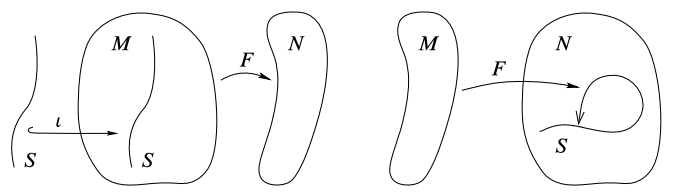
\includegraphics[scale = 0.4]{restricting_domain.png}}
\end{minipage}
\caption{\footnotesize{\textbf{(Left) Restricting the domain. (Right) Restricting the codomain.  \citep{lee2003introduction}}}}
\label{fig: restricting_domain}
\end{figure}

\item The next theorem gives sufficient conditions for a map to be smooth when its codomain is restricted to an immersed submanifold.It shows that the failure of continuity is the only thing that can go wrong.
\begin{theorem} (\textbf{Restricting the Codomain of a Smooth Map}). \citep{lee2003introduction}\\ 
Suppose $M$ is a smooth manifold (without boundary), $S \subseteq M$ is an \textbf{immersed submanifold}, and $F: N \rightarrow M$ is a smooth map whose \textbf{image is contained in $S$}. If $F$ is \textbf{continuous} as a map from $N$ to $S$, then $F: N \rightarrow S$ is smooth.
\end{theorem}

\item \begin{corollary} (\textbf{Embedded Case}). \\
Let $M$ be a smooth manifold and $S \subseteq M$ be an \textbf{embedded submanifold}. Then every smooth map $F: N \rightarrow M$ whose \textbf{image is
contained in $S$} is also \textbf{smooth} as a map from $N$ to $S$.
\end{corollary}

\item \begin{definition}
If $M$ is a smooth manifold and $S \subseteq M$ is an immersed submanifold, then $S$ is said to be \underline{\emph{\textbf{weakly embedded}}} in $M$ if every smooth map $F: N \rightarrow M$ \emph{\textbf{whose image lies in $S$}} is \textbf{\emph{smooth}} as a map from $N$ to $S$. (\emph{Weakly embedded submanifolds} are called \emph{\textbf{initial submanifolds}} by some authors.) 
\end{definition}

\item \begin{remark}
Corollary above shows that \emph{every embedded submanifold is weakly embedded}.
\end{remark}
\end{itemize}
\subsection{Uniqueness of Smooth Structures on Submanifolds}
\begin{itemize}
\item \begin{theorem}
Suppose $M$ is a smooth manifold and $S \subseteq M$ is an \textbf{embedded submanifold}. The subspace topology on $S$ and the smooth structure from the local $k$-slice condition are \textbf{the only topology and smooth structure} with respect to which $S$ is an embedded or immersed submanifold.
\end{theorem}

\item \begin{remark}
Thanks to this uniqueness result, we now know that a \emph{subset} $S \subseteq M$ is an \emph{embedded submanifold} \emph{\textbf{if and only if}} it satisfies \emph{the local slice condition}, and if so, its topology and smooth structure are \emph{\textbf{uniquely determined}}.

Because the local slice condition is \emph{\textbf{a local condition}}, if every point $p \in S$ has a neighborhood \underline{$U \subseteq M$} such that \underline{$U \cap S$} is an embedded $k$-submanifold \underline{\emph{of $U$}}, then $S$ is an embedded $k$-submanifold of $M$.
\end{remark}

\item \begin{theorem}
Suppose $M$ is a smooth manifold and $S \subseteq M$ is an \textbf{immersed submanifold}. For the \textbf{given topology} on $S$, there is \textbf{only one smooth structure} making $S$ into an immersed submanifold.
\end{theorem}

\item \begin{theorem} If $M$ is a smooth manifold and $S \subseteq M$ is a \textbf{weakly embedded submanifold}, then $S$ has \textbf{only one topology and smooth structure} with respect to which it is an immersed submanifold.
\end{theorem}
\end{itemize}
\subsection{Extending Functions from Submanifolds}
\begin{itemize}
\item \begin{remark}
Complementary to the restriction problem is the problem of extending smooth functions from a submanifold to the ambient manifold. Here we say $f \in \cC^{\infty}(S)$ for submanifold $S\subseteq M$, when $f$ is considered as a function on the manifold $S$.
\end{remark}

\item \begin{lemma} (\textbf{Extension Lemma for Functions on Submanifolds}). \\
Suppose $M$ is a smooth manifold, $S\subseteq M$ is a smooth submanifold, and $f \in \cC^{\infty}(S)$.
\begin{enumerate}
\item  If $S$ is \textbf{embedded}, then there exist a \textbf{neighborhood} $U$ of $S$ in $M$ and a smooth
function $\widetilde{f} \in  \cC^{\infty}(U)$ such that $\widetilde{f}|_{S} = f$.
\item If $S$ is \textbf{properly embedded}, then the neighborhood U above can be taken to be \textbf{all} of $M$. 
\end{enumerate}
\end{lemma}
\end{itemize}

\section{The Tangent Space to a Submanifold}
\begin{itemize}
\begin{figure}
\begin{minipage}[htb]{1\linewidth}
  \centering
  \centerline{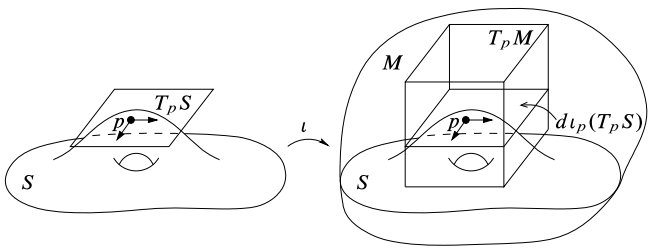
\includegraphics[scale = 0.4]{tangent_space_subman.png}}
\end{minipage}
\caption{\footnotesize{\textbf{The tangent space of a submanifold.  \citep{lee2003introduction}}}}
\label{fig: tangent_space_subman}
\end{figure}

\item \begin{remark}
The \emph{\textbf{tangent space to a smooth submanifold}} of an abstract smooth manifold can be viewed as \emph{a \textbf{subspace}} of \emph{\textbf{the tangent space to the ambient manifold}}, once we make appropriate identifications. The following proof is based on the \underline{\emph{\textbf{differential}}} of \underline{\emph{\textbf{the inclusion map}}} as a smooth immersion.
\end{remark}
\begin{proof} 
Let $M$ be a smooth manifold with or without boundary, and let $S\subseteq M$ be an immersed or embedded submanifold. Since the inclusion map $\iota: S \xhookrightarrow{} M$ is a \emph{\textbf{smooth immersion}}, at each point $p \in S$ we have an \emph{injective linear map} $d\iota_{p}: T_{p}S \rightarrow T_{p}M$.
In terms of \emph{\textbf{derivations}}, this injection works in the following way: for any vector $v \in T_{p}S$, the image vector $\widetilde{v} = d\iota_{p}(v) \in T_{p}M$ acts on smooth functions on $M$ by
\begin{align*}
\widetilde{v}f = d\iota_{p}(v)f = v\paren{f \circ \iota} = v\paren{f|_{S}}.
\end{align*}
We adopt the convention of \emph{\textbf{identifying}} $T_{p}S$ with \emph{\textbf{its image} under this map}, thereby
thinking of $T_{p}S$ as a certain linear subspace of $T_{p}M$ (Fig. \ref{fig: tangent_space_subman}). This identification makes sense regardless of whether $S$ is \emph{embedded or immersed}. \qed
\end{proof}


\item There are several \emph{alternative} ways to \emph{characterize} the tangent space of a submanifold 
\begin{enumerate}
\item \underline{\emph{\textbf{Smooth curve} on \textbf{submanifold}}}. 
\begin{proposition}
Suppose $M$ is a smooth manifold with or without boundary, $S\subseteq M$ is an immersed or embedded submanifold, and $p \in S$. A vector $v \in T_{p}M$ is
in $T_{p}S$ if and only if there is a smooth curve  $\gamma: J \rightarrow M$ whose \textbf{image is contained in $S$}, and which is also \textbf{smooth} as a map into $S$, such that $0 \in J$, $\gamma(0) = p$, and $\gamma'(0) = v$.
\end{proposition}

\item \emph{\textbf{Derivations} on \underline{functions whose \textbf{restriction on submanifold are constant zero}}}.
\begin{proposition}
Suppose $M$ is a smooth manifold, $S\subseteq M$ is an embedded submanifold, and $p \in S$. As a subspace of $T_{p}M$, the tangent space $T_{p}S$ is characterized
by
\begin{align*}
T_{p}S &= \set{v \in T_{p}M: vf = 0\text{ \textbf{whenever} }f \in \cC^{\infty}(M)\text{ \textbf{and} }f|_{S} = 0}.
\end{align*}
\end{proposition}

\item \underline{\emph{\textbf{Kernel subspace} of \textbf{differential map of local defining map}}}.
\begin{proposition}
Suppose $M$ is a smooth manifold and $S \subseteq M$ is an embedded submanifold. If $\Phi: U \rightarrow N$ is any \textbf{local defining map} for $S$, then $T_{p}S = 
\text{\textbf{Ker} }(d\Phi_{p}): T_{p}M \rightarrow T_{\Phi(p)}N$ for each $p \in S \cap U$.
\end{proposition} Note that $S\cap U = (\Phi \circ \iota)^{-1}(c)$ is the level set of $\Phi \circ \iota$ thus it is constant for $\Phi \circ \iota$. So $d\Phi_p \circ d\iota_p = 0$.

\begin{corollary}
Suppose $S \subseteq M$ is a \textbf{level set} of a \textbf{smooth submersion} $\Phi = (\Phi^1,\ldots,\Phi^k): M \rightarrow \bR^k$. A vector $v \in T_{p}M$ is tangent to $S$ if and only if $v\Phi^1 = \ldots = v\Phi^k = 0$.
\end{corollary}
\end{enumerate}

\begin{figure}
\begin{minipage}[htb]{1\linewidth}
  \centering
  \centerline{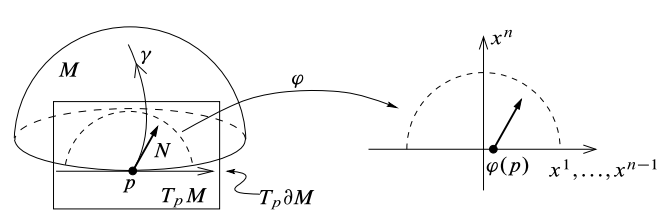
\includegraphics[scale = 0.4]{inward_pointing_vector.png}}
\end{minipage}
\caption{\footnotesize{\textbf{An inward-pointing vector.  \citep{lee2003introduction}}}}
\label{fig: inward_pointing_vector}
\end{figure}

\item \begin{remark}
If $M$ is a smooth manifold \emph{\textbf{with boundary}} and $p \in \partial M$, it is intuitively evident
that the vectors in $T_{p}M$ can be separated into \emph{\textbf{three classes}}:  
\begin{enumerate}
\item those \emph{\textbf{tangent to the boundary}};
\item those pointing \emph{\textbf{inward}}; See Fig \ref{fig: inward_pointing_vector}.
\item those pointing \emph{\textbf{outward}}.
\end{enumerate}
\end{remark}

\begin{definition}
If $p \in \partial M$, a vector $v \in T_{p}M \setminus T_{p}\partial M$ is said to be \emph{\textbf{inward-pointing}} if for some $\epsilon > 0$ there exists a smooth curve $\gamma: [0, \epsilon)\rightarrow M$ such that $\gamma(0) = p$ and $\gamma'(0) = v$, and it is \emph{\textbf{outward-pointing}} if there exists such a curve whose domain is $(-\epsilon, 0]$.
\end{definition}

\begin{proposition} (\textbf{Characterization of Tangent Vectors on Boundary using Component Functions})\\
Suppose $M$ is a smooth $n$-dimensional manifold with boundary, $p \in \partial M$, and $(x^i)$ are any smooth boundary coordinates defined on a neighborhood of $p$. The \textbf{inward-pointing vectors} in $T_{p}M$ are precisely those with \textbf{positive $x^n$-component}, the \textbf{outward-pointing} ones are those with \textbf{negative $x^n$-component}, and the ones \textbf{tangent to $\partial M$} are those with \textbf{zero $x^n$-component}. Thus, $T_{p}M$ is the \textbf{disjoint union} of $T_{p}\partial M$, the set of inward-pointing vectors, and the set of outwardpointing vectors, and $v \in T_{p}M$ is inward-pointing if and only if $-v$ is outward-pointing.
\end{proposition}

\item \begin{definition}
If $M$ is a smooth manifold with boundary, a \emph{\textbf{boundary defining function}} for $M$ is a smooth function $f: M \rightarrow [0, \infty)$ such that $f^{-1}(0) = \partial M$ and $df_{p} \neq 0$ for all $p \in \partial M$. For example, $f(x) =\sqrt{1 - \abs{x}^2}$ is a boundary defining function for the closed unit ball $\overline{\bB}^n$.
\end{definition}

\item \begin{proposition}
Every smooth manifold with boundary admits a \textbf{boundary defining function}.
\end{proposition}
\end{itemize}


\section{Submanifolds with Boundary}




\newpage
\bibliographystyle{plainnat}
\bibliography{book_reference.bib}
\end{document}